%!TEX TS-program = pdflatex
%!TEX root = ../main.tex
%!TEX encoding = UTF-8 Unicode


\section[Introduction]{Introduction}

	\begin{frame}{Contents}
			
		\tableofcontents
		
		\note{
			\dots			
		}		
		
	\end{frame}
	
	\begin{frame}{Audio Segmentation and Sound Event Detection}
	
		The goal of automatic sound event detection (SED) methods is to recognize what is happening in an audio signal and when it is happening\footcite{Mesaros2021SoundED}.
		In practice, the goal is to recognize at what temporal instances different sounds are active within an audio signal.
		An example of sound event detection is presented below.
		
		\begin{figure}
			\centering
			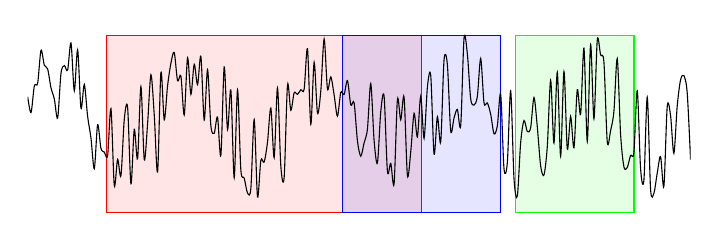
\begin{tikzpicture}[samples=200, domain=0:5*360]
			
				\draw[draw=red,fill=red,fill opacity=0.1] (1,0) rectangle ++(4,2.25);
				\draw[draw=blue,fill=blue,fill opacity=0.1] (4,0) rectangle ++(2,2.25);
				\draw[draw=green,fill=green,fill opacity=0.1] (6.2,0) rectangle ++(1.5,2.25);

        		\begin{axis}[
            		width=10cm, height=4cm,
            		enlarge x limits=false,
            		hide x axis,
            		hide y axis
        		]
        			\addplot [no markers, smooth] {sin(x)+rand*2};
        		\end{axis}
    		\end{tikzpicture}
			\caption{Event Detection in an audio track.}
			\label{fig:sounddetection}
		\end{figure}
		
	\end{frame}
	
	\begin{frame}{Datasets}
	
		Common datasets for Audio Segmentation and Sound Event Detection problems are:
		
		\begin{itemize}
			\item \textbf{TUT Sound Event Detection}: primarily consists of street recordings with traffic and other activity, with audio examples of \SI{2.56}{\second} and a total size of approximately \SI{1.5}{\hour}. It has six unique audio classes -- Brakes Squeaking, Car, Children, Large Vehicle, People Speaking, and People Walking;
			\item \textbf{Urban-SED}: purely synthetic dataset, with audio example of \SI{10}{\second} and a total size of about \SI{30}{\hour}. It has ten unique audio classes -- Air Conditioner, Car Horn, Children Playing, Dog Bark, Drilling, Engine Idling, Gun Shot, Jackhammer, Siren, and Street Music.
		\end{itemize}
		
		The first dataset is too small to train a Deep Neural Network model and requires use of augmentation techniques (like \textbf{SpecAugment}\footcite{park19e_interspeech}).

	\end{frame}
	
	\begin{frame}[allowframebreaks]{Metrics}
	
		A popular toolbox for Sound Event Detection models evaluation is \textbf{SED Eval}\footcite{app6060162}.
		
		The \textbf{F$_{1}$-score} for a SED model prediction is defined as:
		\vspace{-3em}
		\begin{multicols}{2}
  			\begin{equation*}
    			\text{P} = \frac{\text{TP}}{\text{TP} + \text{FP}}
  			\end{equation*}\break
  			\begin{equation*}
    			\text{R} = \frac{\text{TP}}{\text{TP} + \text{FN}}
  			\end{equation*}
		\end{multicols}
		\vspace{-1em}
		\begin{equation*}
			\text{F$_{1}$-score} = 2 \times \frac{\text{P} \times \text{R}}{\text{P} + \text{R}}
		\end{equation*}
		
		where TP, FP and FN are respectively (for each audio segment):
		\begin{itemize}
			\item the ground truth and system output both indicate an event to be active;
			\item the ground truth indicates an event to be inactive, but the system as active;
			\item the ground truth indicates an event to be active, but the system as inactive.
		\end{itemize}
		
		\framebreak
		
		The \textbf{Error rate} keeps in consideration \textit{Substitutions}, \textit{Insertions}, and \textit{Deletions}:\vspace{-1em}
		
		\begin{multicols}{2}		
  			\begin{equation*}
    			S(k)=\min(\text{FN}(k),\text{FP}(k))
  			\end{equation*}
  			\begin{equation*}
    			D(k)=\max(0,\text{FN}(k)-\text{FP}(k))
  			\end{equation*}
  			\begin{equation*}
    			I(k)=\max(0,\text{FP}(k)-\text{FN}(k))
  			\end{equation*}
			\break
  			\begin{equation*}
    			\text{ER}=\frac{\sum_{k=1}^{K}S(k)+\sum_{k=1}^{K}D(k)+\sum_{k=1}^{K}I(k)}{\sum_{k=1}^{K}N(k)}
  			\end{equation*}
		\end{multicols}

		\begin{figure}
			\centering
			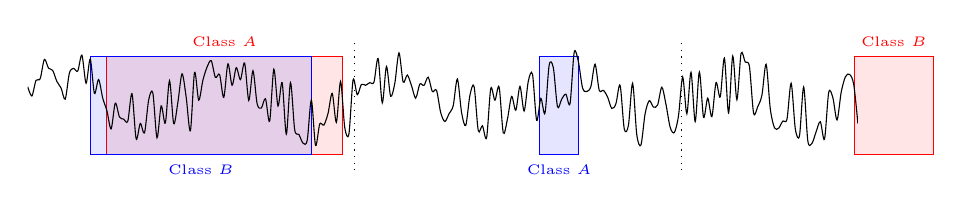
\begin{tikzpicture}[samples=200, domain=0:5*360]
			
				\draw[dotted] (4.15,-.2) -- (4.15,1.45);
				\draw[dotted] (8.3,-.2) -- (8.3,1.45);
			
				
				\draw[draw=red,fill=red,fill opacity=0.1] (1,0) rectangle ++(3,1.25);
				\node[above] at (2.5,1.25) {\tiny \textcolor{red}{Class $A$}};
				\draw[draw=red,fill=red,fill opacity=0.1] (10.5,0) rectangle ++(1,1.25);
				\node[above] at (11.0,1.25) {\tiny \textcolor{red}{Class $B$}};

				\draw[draw=blue,fill=blue,fill opacity=0.1] (.8,0) rectangle ++(2.8,1.25);
				\node[below] at (2.2,0) {\tiny \textcolor{blue}{Class $B$}};
				\draw[draw=blue,fill=blue,fill opacity=0.1] (6.5,0) rectangle ++(0.5,1.25);
				\node[below] at (6.75,0) {\tiny \textcolor{blue}{Class $A$}};

        		\begin{axis}[
            		width=\textwidth, height=3cm,
            		enlarge x limits=false,
            		hide x axis,
            		hide y axis
        		]
        			\addplot [no markers, smooth] {sin(x)+rand*2};
        		\end{axis}
    		\end{tikzpicture}\vspace{-0.75em}
			\caption{Example of \textcolor{red}{ground truth} and model \textcolor{blue}{predicted labels} in three segments.}
			\label{fig:metrics}
		\end{figure}


	\end{frame}
	
